\documentclass[10pt,a4paper,oneside]{article}
\usepackage[utf8]{inputenc}
\usepackage[english]{babel}
\usepackage{forloop}
\usepackage{amsmath}
\usepackage{amsfonts}
\usepackage{amssymb}
\usepackage{gensymb}
\usepackage{graphicx}
\usepackage[dvipsnames]{xcolor}
\usepackage{tikz}
\usetikzlibrary{arrows,automata,shapes}
\tikzstyle{decision} = [diamond, draw, fill=blue!20, text width=4.5em, text badly centered, node distance=2.5cm, inner sep=0pt]
\tikzstyle{block} = [rectangle, draw, fill=blue!20, text width=5em, text centered, rounded corners, minimum height=4em]
\tikzstyle{line} = [draw, very thick, color=black!50, -latex']
\tikzstyle{cloud} = [draw, ellipse,fill=red!20, node distance=2.5cm,minimum height=2em]
\usepackage[siunitx]{circuitikz}

\definecolor{LightGray}{gray}{0.9}
\definecolor{NormalGray}{gray}{0.8}
\definecolor{DarkGray}{gray}{0.7}

\title{Libre Silicon process specification}
\date{\today} 
\author{David Lanzendörfer}

\begin{document}
\maketitle

\begin{abstract}
	Copyright © 2017 LANCEVILLE TECHNOLOGY GROUP CO., LIMITED. All rights reserved. \\

	This process is licensed under the Libre Silicon public license; you can redistribute it and/or modify it under the terms of the Libre Silicon public license
	as published by the Libre Silicon alliance, either version 1 of the License, or (at your option) any later version.

	This design is distributed in the hope that it will be useful, but WITHOUT ANY WARRANTY; without even the implied warranty of MERCHANTABILITY or FITNESS FOR A PARTICULAR PURPOSE.
	See the Libre Silicon Public License for more details. \\

	This is the specification of the free silicon manufacturing standard for manufacturing the ls180nm\footnotemark standard logic cells and related free technology nodes from the LibreSilicon project.
	\footnotetext[1]{https://github.com/leviathanch/ls180nm}
\end{abstract}
\newpage

\section{Discrete components}
This basic initial process draft is CMOS only and for this reason only consists the two MOSFET typed n/p required to build CMOS technology.
Resistors are not included within this initial process draft.

\subsection{NMOS}
The following circuit symbol will be used throughout the document for symbolizing a NMOS transistor
\begin{center}
	\begin{circuitikz}
		\node at (5,0) [ground] (gnd) {};
		\node at (5,2) [nigfete] (nmos) {} ;
		\node at (4.5,5) [right] (vdd) {$V_{DD}$};
		\draw (gnd) to (nmos.S);
		\draw (nmos.D) to (5,2.5) [R] to (vdd);
		\draw (gnd) to +(-1,0) [vsourcesquare] to (nmos.G);
		\node at (3.9,2.0) {Gate};
		\node at (5.6,2.5) {Drain};
		\node at (5.6,1.5) {Source};
	\end{circuitikz}
\end{center}

The geometry in silicon is being shown below
\begin{center}
	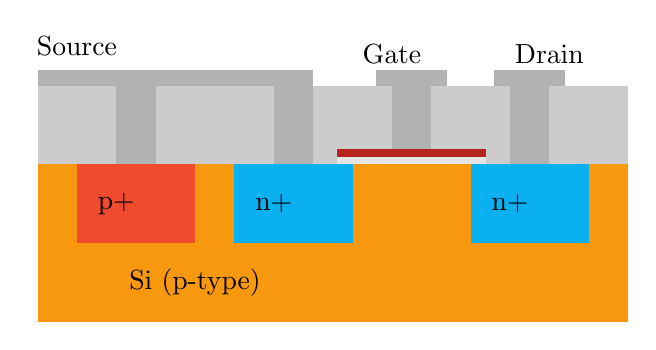
\begin{tikzpicture}
		% substrate
		\fill[YellowOrange] (0,0) rectangle (7.5,2);
		\node at (2,0.5) {Si (p-type)};
		% body
		\fill[RedOrange] (0.5,1) rectangle (2,2);
		\node at (1,1.5) {p+};
		% source
		\fill[ProcessBlue] (2.5,1) rectangle (4,2);
		\node at (3,1.5) {n+};
		% drain
		\fill[ProcessBlue] (5.5,1) rectangle (7,2);
		\node at (6,1.5) {n+};
		%% gate:
		% gate oxide
		\fill[LightGray] (3.8,2) rectangle (5.7,2.1);
		% gate poly
		\fill[BrickRed] (3.8,2.1) rectangle (5.7,2.2);
		% metals ground
		\fill[DarkGray] (1,2) rectangle (1.5,3);
		\fill[DarkGray] (3,2) rectangle (3.5,3);
		\fill[DarkGray] (0,3) rectangle (3.5,3.2); % connection pad GND

		\fill[DarkGray] (4.5,2.2) rectangle (5,3);
		\fill[DarkGray] (4.3,3) rectangle (5.2,3.2); % connection pad VG

		\fill[DarkGray] (6,2) rectangle (6.5,3);
		\fill[DarkGray] (5.8,3) rectangle (6.7,3.2); % connection pad VDD

		% isolation oxides:
		\fill[NormalGray] (0,2) rectangle (1,3);
		\fill[NormalGray] (1.5,2) rectangle (3,3);
		\fill[NormalGray] (3.5,2) rectangle (3.8,3);
		\fill[NormalGray] (3.8,2.2) rectangle (4.5,3);
		\fill[NormalGray] (5,2.2) rectangle (5.7,3);
		\fill[NormalGray] (5.7,2) rectangle (6,3);
		\fill[NormalGray] (6.5,2) rectangle (7.5,3);
		
		\node at (0.5,3.5) {Source};
		\node at (4.5,3.4) {Gate};
		\node at (6.5,3.4) {Drain};
	\end{tikzpicture}
\end{center}

\newpage

\subsection{PMOS}
The following circuit symbol will be used throughout the document for symbolizing a PMOS transistor
\begin{center}
	\begin{circuitikz}
		\node at (5,0) [ground] (gnd) {};
		\node at (5,2) [pigfete,xscale=1,yscale=-1] (pmos) {} ;
		\node at (4.5,5) [right] (vdd) {$V_{DD}$};
		\draw (gnd) to (pmos.S);
		\draw (pmos.D) to (5,2.5) [R] to (vdd);
		\draw (gnd) to +(-1,0) [vsourcesquare] to (pmos.G);
		\node at (3.9,2.0) {Gate};
		\node at (5.6,2.5) {Drain};
		\node at (5.6,1.5) {Source};
	\end{circuitikz}
\end{center}

The geometry in silicon is being shown below
\begin{center}
	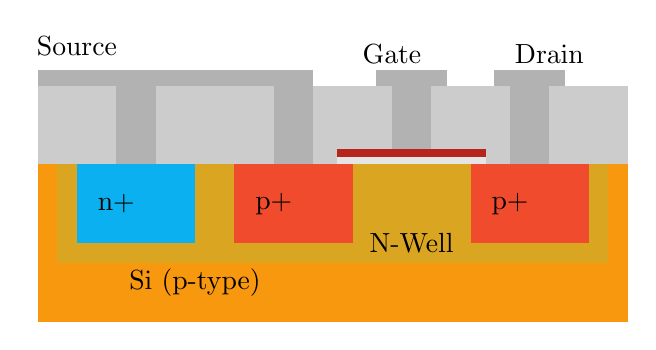
\begin{tikzpicture}
		% substrate
		\fill[YellowOrange] (0,0) rectangle (7.5,2);
		\node at (2,0.5) {Si (p-type)};

		% n-well
		\fill[Goldenrod] (0.25,0.75) rectangle (7.25,2);
		\node at (4.75,1) {N-Well};

		% body
		\fill[ProcessBlue] (0.5,1) rectangle (2,2);
		\node at (1,1.5) {n+};
		% source
		\fill[RedOrange] (2.5,1) rectangle (4,2);
		\node at (3,1.5) {p+};
		% drain
		\fill[RedOrange] (5.5,1) rectangle (7,2);
		\node at (6,1.5) {p+};
		%% gate:
		% gate oxide
		\fill[LightGray] (3.8,2) rectangle (5.7,2.1);
		% gate poly
		\fill[BrickRed] (3.8,2.1) rectangle (5.7,2.2);
		% metals ground
		\fill[DarkGray] (1,2) rectangle (1.5,3);
		\fill[DarkGray] (3,2) rectangle (3.5,3);
		\fill[DarkGray] (0,3) rectangle (3.5,3.2); % connection pad GND

		\fill[DarkGray] (4.5,2.2) rectangle (5,3);
		\fill[DarkGray] (4.3,3) rectangle (5.2,3.2); % connection pad VG

		\fill[DarkGray] (6,2) rectangle (6.5,3);
		\fill[DarkGray] (5.8,3) rectangle (6.7,3.2); % connection pad VDD

		% isolation oxides:
		\fill[NormalGray] (0,2) rectangle (1,3);
		\fill[NormalGray] (1.5,2) rectangle (3,3);
		\fill[NormalGray] (3.5,2) rectangle (3.8,3);
		\fill[NormalGray] (3.8,2.2) rectangle (4.5,3);
		\fill[NormalGray] (5,2.2) rectangle (5.7,3);
		\fill[NormalGray] (5.7,2) rectangle (6,3);
		\fill[NormalGray] (6.5,2) rectangle (7.5,3);
		
		\node at (0.5,3.5) {Source};
		\node at (4.5,3.4) {Gate};
		\node at (6.5,3.4) {Drain};
	\end{tikzpicture}
\end{center}

\newpage

\section{CMOS example}
The example which will be used for showing the process steps will be a simple CMOS inverter of which the schematics are drawn below
\begin{center}
	\begin{circuitikz}
		\node at (5,0) [ground] (gnd) {};
		\node at (5,2) [nigfete] (nmos) {} ;
		\node at (5,4) [pigfete] (pmos) {} ;
		\node at (4.5,7) [right] (vdd) {$V_{DD}$};
		\draw (gnd) to (nmos.S);
		\draw (pmos.S) to (5,4.5) [R] to (vdd);
		\draw (gnd) to +(-2,0) [vsourcesquare] to (3,1.75);
		\node at (3.9,2.0) {Gate};
		\node at (5.6,2.5) {Drain};
		\node at (5.6,1.5) {Source};
		\draw (nmos.G) to (3,1.75) to (3,4.275) to (pmos.G);
		\node at (3.9,4.0) {Gate};
		\node at (5.6,3.5) {Drain};
		\node at (5.6,4.5) {Source};
		\draw (pmos.D) to (nmos.D) to (7,2.75) to (7,1.75) [R] to (7,0);
		\draw (7,0) to (gnd);
	\end{circuitikz}
\end{center}

Below the cross section view of the inverter circuitry can be seen.
For the run through of this process we will use this cross section diagram as reference.
\begin{center}
	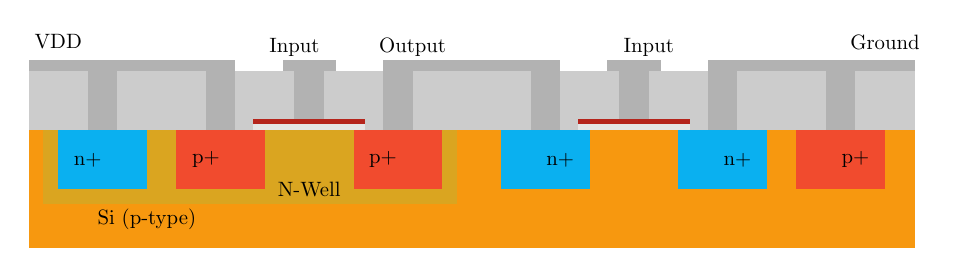
\begin{tikzpicture}[node distance = 3cm, auto, thick,scale=0.75, every node/.style={transform shape}]
		% substrate
		\fill[YellowOrange] (0,0) rectangle (15,2);
		\node at (2,0.5) {Si (p-type)};

		% n-well
		\fill[Goldenrod] (0.25,0.75) rectangle (7.25,2);
		\node at (4.75,1) {N-Well};

		% body
		\fill[ProcessBlue] (0.5,1) rectangle (2,2);
		\node at (1,1.5) {n+};
		% source
		\fill[RedOrange] (2.5,1) rectangle (4,2);
		\node at (3,1.5) {p+};
		% drain
		\fill[RedOrange] (5.5,1) rectangle (7,2);
		\node at (6,1.5) {p+};

		%% gate:
		% gate oxide
		\fill[LightGray] (3.8,2) rectangle (5.7,2.1);
		% gate poly
		\fill[BrickRed] (3.8,2.1) rectangle (5.7,2.2);

		% metals ground
		\fill[DarkGray] (1,2) rectangle (1.5,3);
		\fill[DarkGray] (3,2) rectangle (3.5,3);
		\fill[DarkGray] (0,3) rectangle (3.5,3.2); % connection pad GND

		\fill[DarkGray] (4.5,2.2) rectangle (5,3);
		\fill[DarkGray] (4.3,3) rectangle (5.2,3.2); % connection pad VG

		\fill[DarkGray] (6,2) rectangle (6.5,3);

		% isolation oxides:
		\fill[NormalGray] (0,2) rectangle (1,3);
		\fill[NormalGray] (1.5,2) rectangle (3,3);
		\fill[NormalGray] (3.5,2) rectangle (3.8,3);
		\fill[NormalGray] (3.8,2.2) rectangle (4.5,3);
		\fill[NormalGray] (5,2.2) rectangle (5.7,3);
		\fill[NormalGray] (5.7,2) rectangle (6,3);
		\fill[NormalGray] (6.5,2) rectangle (7.5,3);

		%%% nmos:
		% body
		\fill[RedOrange] (13,1) rectangle (14.5,2);
		\node at (14,1.5) {p+};
		% source
		\fill[ProcessBlue] (11,1) rectangle (12.5,2);
		\node at (12,1.5) {n+};
		% drain
		\fill[ProcessBlue] (8,1) rectangle (9.5,2);
		\node at (9,1.5) {n+};
		%% gate:
		% gate oxide
		\fill[LightGray] (9.3,2) rectangle (11.2,2.1);
		% gate poly
		\fill[BrickRed] (11.2,2.1) rectangle (9.3,2.2);

		% metals ground
		\fill[DarkGray] (13.5,2) rectangle (14,3);
		\fill[DarkGray] (11.5,2) rectangle (12,3);
		\fill[DarkGray] (11.5,3) rectangle (15,3.2); % connection pad GND
		
		\fill[DarkGray] (10,2.2) rectangle (10.5,3);
		\fill[DarkGray] (9.8,3) rectangle (10.7,3.2); % connection pad VG
		
		\fill[DarkGray] (8.5,2) rectangle (9,3);
		\fill[DarkGray] (6,3) rectangle (9,3.2); % connection pad VDD

		% isolation oxides:
		\fill[NormalGray] (14,2) rectangle (15,3);
		\fill[NormalGray] (12,2) rectangle (13.5,3);
		\fill[NormalGray] (11.2,2) rectangle (11.5,3);
		\fill[NormalGray] (10.5,2.2) rectangle (11.2,3);
		\fill[NormalGray] (9.3,2.2) rectangle (10,3);
		\fill[NormalGray] (9,2) rectangle (9.3,3);
		\fill[NormalGray] (7.5,2) rectangle (8.5,3);

		\node at (0.5,3.5) {VDD};
		\node at (14.5,3.5) {Ground};
		\node at (4.5,3.4) {Input};
		\node at (10.5,3.4) {Input};
		\node at (6.5,3.4) {Output};
	\end{tikzpicture}
\end{center}

\newpage
\section{Process}
Below the general flow chart of the overall process flow can be seen. These process steps will be discussed within the following sections.
\begin{center}
	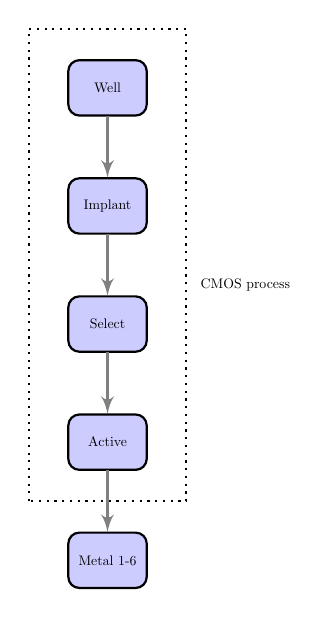
\begin{tikzpicture}[node distance = 3cm, auto, thick,scale=0.5, every node/.style={transform shape}]
		% Place nodes
		\node [block] (well) {Well};
		\node [block, below of=well] (implant) {Implant};
		\node [block, below of=implant] (select) {Select};
		\node [block, below of=select] (active) {Active};
		\node [block, below of=active] (metal) {Metal 1-6};
		% Draw edges
		\path [line] (well) -- (implant);
		\path [line] (implant) -- (select);
		\path [line] (select) -- (active);
		\path [line] (active) -- (metal);
		
		\draw[dotted] (-2,-10.5) rectangle (2,1.5);
		\node at (3.5,-5) {CMOS process};
	\end{tikzpicture}
\end{center}
The four starting overall process steps are part of an overall active part of the technology, while the final metal (respectively contact) layers will be used for making a contact between the logic gates and macro cells and making them available to the exterior world.
For this process p-substrate is the required basic substrate, but forks and modifications will be very well possible based on a Graphene substrate or alike, still under the LSPL.
The decision to use an n-well approach is based largely on the compatibility with the existing nMOS process.
The starting material is a p-type, <100> oriented silicon with a doping concentration of $\approx 9\times10^{14}cm^{-3}$.

\newpage

\subsection{Well}
In order to build CMOS (Complementary metal–oxide–semiconductor/P and N MOS) on the same substrate an n-well is required for building the complementary P-channel transistor for a n-p-channel logic circuitry as shown above in the example section.
The n-well will serve us as an island of n-doped substrate within the p-doped basis substrate.
The cross section as well as the top view of the targeted geometry are shown below.

\begin{center}
	
\begin{tikzpicture}[node distance = 3cm, auto, thick,scale=0.3, every node/.style={transform shape}]
		% substrate
		\fill[YellowOrange] (0,0) rectangle (15,2);
		\node at (2,0.5) {Si (p-type)};
		% n-well
		\fill[Goldenrod] (0.25,0.75) rectangle (7.25,2);
		\node at (4.75,1) {N-Well};
	\end{tikzpicture}
	
\begin{tikzpicture}[node distance = 3cm, auto, thick,scale=0.2, every node/.style={transform shape}]
		% resist
		\fill[YellowOrange] (0,0) rectangle (15,10);
		% substrate
		\fill[Goldenrod] (0.25,0.5) rectangle (7.25,9.5);
	\end{tikzpicture}
\end{center}

\subsubsection{Dioxide layer}
In order to selectively inject charge carrying atoms into the crystalline structure a protective dioxide ($SiO_2$) layer needs to be grown on top of a p-type substrate.
\begin{center}
	
\begin{tikzpicture}[node distance = 3cm, auto, thick,scale=0.3, every node/.style={transform shape}]
		% substrate
		\fill[YellowOrange] (0,0) rectangle (15,2);
		\node at (2,0.5) {Si (p-type)};
	\end{tikzpicture}

	
\includegraphics[scale=0.01]{down_arrow.png}

	
\begin{tikzpicture}[node distance = 3cm, auto, thick,scale=0.3, every node/.style={transform shape}]
		% substrate
		\fill[YellowOrange] (0,0) rectangle (15,2);
		\node at (2,0.5) {Si (p-type)};
		% oxide
		\fill[gray] (0,2) rectangle (15,2.6);
		\node at (2,2.1) {SiO2};
	\end{tikzpicture}
\end{center}
There is no clear general equation perfectly describing the absorption behavior of silicon dioxide but the industrial best practice is a layer of around (500nm$\approx$5000\normalfont\AA) thickness or more.
For this purpose the wafer is being oxidized for at least 90 minutes at 1000\degree C using wet oxidation which results in a dioxide layer at least 500nm($\approx$5000\normalfont\AA) in thickness.

\subsubsection{Patterning and etching}
\begin{center}
	
\begin{tikzpicture}[node distance = 3cm, auto, thick,scale=0.2, every node/.style={transform shape}]
		% substrate
		\fill[YellowOrange] (0,0) rectangle (15,2);
		\node at (2,0.5) {Si (p-type)};
		% oxide
		\fill[gray] (0,2) rectangle (15,2.6);
		% resist
		\fill[orange] (0,2.6) rectangle (15,3.2);
	\end{tikzpicture}
	
\begin{tikzpicture}[node distance = 3cm, auto, thick,scale=0.2, every node/.style={transform shape}]
		% resist
		\fill[orange] (0,0) rectangle (15,10);
	\end{tikzpicture}

	
\includegraphics[scale=0.01]{down_arrow.png}

	
\begin{tikzpicture}[node distance = 3cm, auto, thick,scale=0.2, every node/.style={transform shape}]
		% substrate
		\fill[YellowOrange] (0,0) rectangle (15,2);
		\node at (2,0.5) {Si (p-type)};
		% oxide
		\fill[gray] (0,2) rectangle (15,2.6);
		% resist
		\fill[orange] (0,2.6) rectangle (0.25,3.2);
		\fill[orange] (7.25,2.6) rectangle (15,3.2);
	\end{tikzpicture}
	
\begin{tikzpicture}[node distance = 3cm, auto, thick,scale=0.2, every node/.style={transform shape}]
		% resist
		\fill[orange] (0,0) rectangle (15,10);
		% substrate
		\fill[gray] (0.25,0.5) rectangle (7.25,9.5);
	\end{tikzpicture}

	
\includegraphics[scale=0.01]{down_arrow.png}

	
\begin{tikzpicture}[node distance = 3cm, auto, thick,scale=0.2, every node/.style={transform shape}]
		% substrate
		\fill[YellowOrange] (0,0) rectangle (15,2);
		\node at (2,0.5) {Si (p-type)};
		% oxide
		\fill[gray] (0,2) rectangle (0.25,2.6);
		\fill[gray] (7.25,2) rectangle (15,2.6);
		% resist
		\fill[orange] (0,2.6) rectangle (0.25,3.2);
		\fill[orange] (7.25,2.6) rectangle (15,3.2);
	\end{tikzpicture}
	
\begin{tikzpicture}[node distance = 3cm, auto, thick,scale=0.2, every node/.style={transform shape}]
		% resist
		\fill[orange] (0,0) rectangle (15,10);
		% substrate
		\fill[YellowOrange] (0.25,0.5) rectangle (7.25,9.5);
	\end{tikzpicture}
\end{center}
The resist is being deposited using spin coating and then baked depending on the baking time for the specific resist.
The layout for being exposed onto the resist is being extracted from the "nwell" layer within the GDS2 file.
The thickness of the resist layer and the backing duration will variate depending on the specific equipment for which this process will be implemented with.

\subsubsection{Predeposition}
\begin{center}
	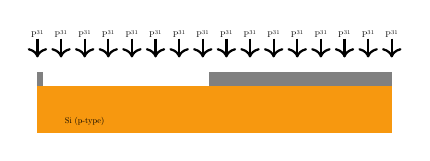
\begin{tikzpicture}[node distance = 3cm, auto, thick,scale=0.3, every node/.style={transform shape}]
		% substrate
		\fill[YellowOrange] (0,0) rectangle (15,2);
		\node at (2,0.5) {Si (p-type)};
		% oxide
		\fill[gray] (0,2) rectangle (0.25,2.6);
		\fill[gray] (7.25,2) rectangle (15,2.6);

		\newcounter{ct}
		\forloop{ct}{0}{\value{ct} < 16}
		{
			\draw [->] (\value{ct},4) -- (\value{ct},3.2);
			\node at (\value{ct},4.2) {P$^{31}$};
		}
	\end{tikzpicture}

	
\includegraphics[scale=0.01]{down_arrow.png}

	
\begin{tikzpicture}[node distance = 3cm, auto, thick,scale=0.3, every node/.style={transform shape}]
		% substrate
		\fill[YellowOrange] (0,0) rectangle (15,2);
		\node at (2,0.5) {Si (p-type)};
		% phosphorus
		\fill[Goldenrod] (0.25,1.8) rectangle (7.25,2);
		\node at (4.75,1.9) {n+};
		% oxide
		\fill[gray] (0,2) rectangle (0.25,2.6);
		\fill[gray] (7.25,2) rectangle (15,2.6);

		\fill[Goldenrod] (0,2.5) rectangle (0.25,2.6);
		\fill[Goldenrod] (7.25,2.5) rectangle (15,2.6);
	\end{tikzpicture}
\end{center}
The n-well is implanted with a $P^{31}$ dose of $2.5\times10^{12}cm^{-2}$ at an energy of 100 KeV.

\subsubsection{Infusion}
\begin{center}
	
\begin{tikzpicture}[node distance = 3cm, auto, thick,scale=0.3, every node/.style={transform shape}]
		% substrate
		\fill[YellowOrange] (0,0) rectangle (15,2);
		\node at (2,0.5) {Si (p-type)};
		% phosphorus
		\fill[Goldenrod] (0.25,1.8) rectangle (7.25,2);
		\node at (4.75,1.9) {n+};
		% oxide
		\fill[gray] (0,2) rectangle (0.25,2.6);
		\fill[gray] (7.25,2) rectangle (15,2.6);

		\fill[Goldenrod] (0,2.5) rectangle (0.25,2.6);
		\fill[Goldenrod] (7.25,2.5) rectangle (15,2.6);
	\end{tikzpicture}

	
\includegraphics[scale=0.01]{down_arrow.png}

	
\begin{tikzpicture}[node distance = 3cm, auto, thick,scale=0.3, every node/.style={transform shape}]
		% substrate
		\fill[YellowOrange] (0,0) rectangle (15,2);
		\node at (2,0.5) {Si (p-type)};
		% phosphorus
		\fill[Goldenrod] (0.25,1.8) rectangle (7.25,2.0);
		\node at (4.75,1.9) {n+};
		% oxide
		\fill[gray] (0,2) rectangle (0.25,2.8);
		\fill[gray] (0.25,2) rectangle (7.25,2.3);
		\fill[gray] (7.25,2) rectangle (15,2.8);
		
		\fill[Goldenrod] (0,2.5) rectangle (0.25,2.6);
		\fill[Goldenrod] (7.25,2.5) rectangle (15,2.6);
	\end{tikzpicture}

	
\includegraphics[scale=0.01]{down_arrow.png}

	
\begin{tikzpicture}[node distance = 3cm, auto, thick,scale=0.3, every node/.style={transform shape}]
		% substrate
		\fill[YellowOrange] (0,0) rectangle (15,2);
		\node at (2,0.5) {Si (p-type)};
		% n-well
		\fill[Goldenrod] (0.25,0.75) rectangle (7.25,2);
		\node at (4.75,1) {N-Well};
		% oxide
		\fill[gray] (0,2) rectangle (0.25,2.8);
		\fill[gray] (0.25,2) rectangle (7.25,2.3);
		\fill[gray] (7.25,2) rectangle (15,2.8);
		
		\fill[Goldenrod] (0,2.5) rectangle (0.25,2.6);
		\fill[Goldenrod] (7.25,2.5) rectangle (15,2.6);
	\end{tikzpicture}
\end{center}
The n-well is then annealed, oxidized (250nm$\approx$2500\normalfont\AA) for 32 minutes at 1000\degree C, and then driven-in for 960 minutes at 1150\degree C in an inert ambient.

\subsubsection{Cleaning}
\begin{center}
	
\begin{tikzpicture}[node distance = 3cm, auto, thick,scale=0.3, every node/.style={transform shape}]
		% substrate
		\fill[YellowOrange] (0,0) rectangle (15,2);
		\node at (2,0.5) {Si (p-type)};
		% n-well
		\fill[Goldenrod] (0.25,0.75) rectangle (7.25,2);
		\node at (4.75,1) {N-Well};
		% oxide
		\fill[gray] (0,2) rectangle (0.25,2.8);
		\fill[gray] (0.25,2) rectangle (7.25,2.3);
		\fill[gray] (7.25,2) rectangle (15,2.8);
		
		\fill[Goldenrod] (0,2.5) rectangle (0.25,2.6);
		\fill[Goldenrod] (7.25,2.5) rectangle (15,2.6);
	\end{tikzpicture}
	
	
\includegraphics[scale=0.01]{down_arrow.png}

	
\begin{tikzpicture}[node distance = 3cm, auto, thick,scale=0.3, every node/.style={transform shape}]
		% substrate
		\fill[YellowOrange] (0,0) rectangle (15,2);
		\node at (2,0.5) {Si (p-type)};
		% n-well
		\fill[Goldenrod] (0.25,0.75) rectangle (7.25,2);
		\node at (4.75,1) {N-Well};
	\end{tikzpicture}
\end{center}
We use hydrofluoric acid, because it doesn't etch silicon at all but is very aggressive towards $SiO_2$

\newpage

\subsection{Active}
\subsubsection{Gate oxide growth}
\begin{center}
	
\begin{tikzpicture}[node distance = 3cm, auto, thick,scale=0.3, every node/.style={transform shape}]
		% substrate
		\fill[YellowOrange] (0,0) rectangle (15,2);
		\node at (2,0.5) {Si (p-type)};
		% n-well
		\fill[Goldenrod] (0.25,0.75) rectangle (7.25,2);
		\node at (4.75,1) {N-Well};
	\end{tikzpicture}

	
\includegraphics[scale=0.01]{down_arrow.png}
	
	
\begin{tikzpicture}[node distance = 3cm, auto, thick,scale=0.3, every node/.style={transform shape}]
		% substrate
		\fill[YellowOrange] (0,0) rectangle (15,2);
		\node at (2,0.5) {Si (p-type)};
		% n-well
		\fill[Goldenrod] (0.25,0.75) rectangle (7.25,2);
		\node at (4.75,1) {N-Well};
		% gate oxide layer
		\fill[LightGray] (0,2) rectangle (15,2.1);
	\end{tikzpicture}
\end{center}

\subsubsection{Polysilicon growth}
\begin{center}
	
\begin{tikzpicture}[node distance = 3cm, auto, thick,scale=0.3, every node/.style={transform shape}]
		% substrate
		\fill[YellowOrange] (0,0) rectangle (15,2);
		\node at (2,0.5) {Si (p-type)};
		% n-well
		\fill[Goldenrod] (0.25,0.75) rectangle (7.25,2);
		\node at (4.75,1) {N-Well};
		% gate oxide layer
		\fill[LightGray] (0,2) rectangle (15,2.1);
	\end{tikzpicture}

	
\includegraphics[scale=0.01]{down_arrow.png}

	
\begin{tikzpicture}[node distance = 3cm, auto, thick,scale=0.3, every node/.style={transform shape}]
		% substrate
		\fill[YellowOrange] (0,0) rectangle (15,2);
		\node at (2,0.5) {Si (p-type)};
		% n-well
		\fill[Goldenrod] (0.25,0.75) rectangle (7.25,2);
		\node at (4.75,1) {N-Well};
		% gate oxide layer
		\fill[LightGray] (0,2) rectangle (15,2.1);
		% poly layer
		\fill[BrickRed] (0,2.1) rectangle (15,2.2);
	\end{tikzpicture}
\end{center}

\subsubsection{Patterning}
\begin{center}
	
\begin{tikzpicture}[node distance = 3cm, auto, thick,scale=0.3, every node/.style={transform shape}]
		% substrate
		\fill[YellowOrange] (0,0) rectangle (15,2);
		\node at (2,0.5) {Si (p-type)};
		% n-well
		\fill[Goldenrod] (0.25,0.75) rectangle (7.25,2);
		\node at (4.75,1) {N-Well};
		% gate oxide layer
		\fill[LightGray] (0,2) rectangle (15,2.1);
		% poly layer
		\fill[BrickRed] (0,2.1) rectangle (15,2.2);
	\end{tikzpicture}

	
\includegraphics[scale=0.01]{down_arrow.png}

	
\begin{tikzpicture}[node distance = 3cm, auto, thick,scale=0.3, every node/.style={transform shape}]
		% substrate
		\fill[YellowOrange] (0,0) rectangle (15,2);
		\node at (2,0.5) {Si (p-type)};
		% n-well
		\fill[Goldenrod] (0.25,0.75) rectangle (7.25,2);
		\node at (4.75,1) {N-Well};
		% gate oxide layer
		\fill[LightGray] (0,2) rectangle (15,2.1);
		% poly layer
		\fill[BrickRed] (0,2.1) rectangle (15,2.2);
		% resist layer
		\fill[orange] (0,2.2) rectangle (15,2.8);
	\end{tikzpicture}

	
\includegraphics[scale=0.01]{down_arrow.png}

	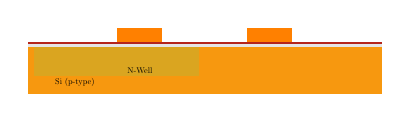
\begin{tikzpicture}[node distance = 3cm, auto, thick,scale=0.3, every node/.style={transform shape}]
		% substrate
		\fill[YellowOrange] (0,0) rectangle (15,2);
		\node at (2,0.5) {Si (p-type)};
		% n-well
		\fill[Goldenrod] (0.25,0.75) rectangle (7.25,2);
		\node at (4.75,1) {N-Well};
		% gate oxide layer
		\fill[LightGray] (0,2) rectangle (15,2.1);
		% poly layer
		\fill[BrickRed] (0,2.1) rectangle (15,2.2);
		% resist
		\fill[orange] (3.8,2.2) rectangle (5.7,2.8);
		\fill[orange] (9.3,2.2) rectangle (11.2,2.8);
	\end{tikzpicture}
\end{center}

\subsubsection{Etching}
\begin{center}
	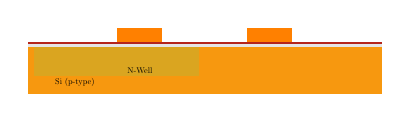
\begin{tikzpicture}[node distance = 3cm, auto, thick,scale=0.3, every node/.style={transform shape}]
		% substrate
		\fill[YellowOrange] (0,0) rectangle (15,2);
		\node at (2,0.5) {Si (p-type)};
		% n-well
		\fill[Goldenrod] (0.25,0.75) rectangle (7.25,2);
		\node at (4.75,1) {N-Well};
		% gate oxide layer
		\fill[LightGray] (0,2) rectangle (15,2.1);
		% poly layer
		\fill[BrickRed] (0,2.1) rectangle (15,2.2);
		% resist
		\fill[orange] (3.8,2.2) rectangle (5.7,2.8);
		\fill[orange] (9.3,2.2) rectangle (11.2,2.8);
	\end{tikzpicture}

	
\includegraphics[scale=0.01]{down_arrow.png}

	
\begin{tikzpicture}[node distance = 3cm, auto, thick,scale=0.3, every node/.style={transform shape}]
		% substrate
		\fill[YellowOrange] (0,0) rectangle (15,2);
		\node at (2,0.5) {Si (p-type)};
		% n-well
		\fill[Goldenrod] (0.25,0.75) rectangle (7.25,2);
		\node at (4.75,1) {N-Well};

		% gate oxide
		\fill[LightGray] (3.8,2) rectangle (5.7,2.1);
		\fill[LightGray] (9.3,2) rectangle (11.2,2.1);
		
		% gate poly
		\fill[BrickRed] (3.8,2.1) rectangle (5.7,2.2);
		\fill[BrickRed] (9.3,2.1) rectangle (11.2,2.2);

		% resist
		\fill[orange] (3.8,2.2) rectangle (5.7,2.8);
		\fill[orange] (9.3,2.2) rectangle (11.2,2.8);
	\end{tikzpicture}

	
\includegraphics[scale=0.01]{down_arrow.png}

	
\begin{tikzpicture}[node distance = 3cm, auto, thick,scale=0.3, every node/.style={transform shape}]
		% substrate
		\fill[YellowOrange] (0,0) rectangle (15,2);
		\node at (2,0.5) {Si (p-type)};
		% n-well
		\fill[Goldenrod] (0.25,0.75) rectangle (7.25,2);
		\node at (4.75,1) {N-Well};

		% gate oxide
		\fill[LightGray] (3.8,2) rectangle (5.7,2.1);
		\fill[LightGray] (9.3,2) rectangle (11.2,2.1);
		
		% gate poly
		\fill[BrickRed] (3.8,2.1) rectangle (5.7,2.2);
		\fill[BrickRed] (9.3,2.1) rectangle (11.2,2.2);
	\end{tikzpicture}
\end{center}
Because the exact shape of the gate contact is required for a reproducible property characterization of the transistor geometry, dry etching is being used for etching the poly-oxide layer stack.

\newpage

\subsection{Implant}
\begin{center}
	
\begin{tikzpicture}[node distance = 3cm, auto, thick,scale=0.3, every node/.style={transform shape}]
		% substrate
		\fill[YellowOrange] (0,0) rectangle (15,2);
		\node at (2,0.5) {Si (p-type)};
		% n-well
		\fill[Goldenrod] (0.25,0.75) rectangle (7.25,2);
		\node at (4.75,1) {N-Well};

		% gate oxide
		\fill[LightGray] (3.8,2) rectangle (5.7,2.1);
		\fill[LightGray] (9.3,2) rectangle (11.2,2.1);
		
		% gate poly
		\fill[BrickRed] (3.8,2.1) rectangle (5.7,2.2);
		\fill[BrickRed] (9.3,2.1) rectangle (11.2,2.2);
	\end{tikzpicture}
\end{center}

\newpage

\subsection{Select}
\begin{center}
	
\begin{tikzpicture}[node distance = 3cm, auto, thick,scale=0.3, every node/.style={transform shape}]
		% substrate
		\fill[YellowOrange] (0,0) rectangle (15,2);
		\node at (2,0.5) {Si (p-type)};
		% n-well
		\fill[Goldenrod] (0.25,0.75) rectangle (7.25,2);
		\node at (4.75,1) {N-Well};

		% gate oxide
		\fill[LightGray] (3.8,2) rectangle (5.7,2.1);
		\fill[LightGray] (9.3,2) rectangle (11.2,2.1);
		
		% gate poly
		\fill[BrickRed] (3.8,2.1) rectangle (5.7,2.2);
		\fill[BrickRed] (9.3,2.1) rectangle (11.2,2.2);
	\end{tikzpicture}
\end{center}

\newpage

\subsection{Metal}
\begin{center}
	
\begin{tikzpicture}[node distance = 3cm, auto, thick,scale=0.3, every node/.style={transform shape}]
		% substrate
		\fill[YellowOrange] (0,0) rectangle (15,2);
		\node at (2,0.5) {Si (p-type)};
		% n-well
		\fill[Goldenrod] (0.25,0.75) rectangle (7.25,2);
		\node at (4.75,1) {N-Well};

		% gate oxide
		\fill[LightGray] (3.8,2) rectangle (5.7,2.1);
		\fill[LightGray] (9.3,2) rectangle (11.2,2.1);
		
		% gate poly
		\fill[BrickRed] (3.8,2.1) rectangle (5.7,2.2);
		\fill[BrickRed] (9.3,2.1) rectangle (11.2,2.2);
	\end{tikzpicture}
\end{center}

\end{document}